\documentclass[tikz,border=2pt]{standalone}
\usepackage{amsmath}
\usetikzlibrary{arrows.meta}
\begin{document}
% Levels of knowledge as nested events: E contains K^1(E), which contains K^2(E), ...; common knowledge
% is what lies in every level. In Example 1, rationality deletes R, K^1 deletes B, K^2 deletes L.
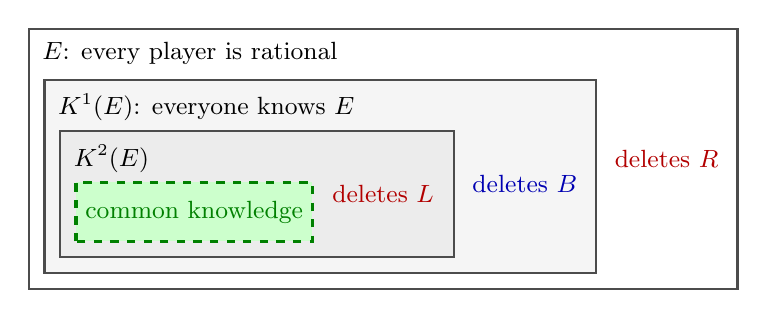
\begin{tikzpicture}[font=\small, >={Latex[length=2mm]}]
  \draw[thick, gray!60!black] (0,0) rectangle (9.0,3.3);
  \draw[thick, gray!60!black, fill=gray!8] (0.2,0.2) rectangle (7.2,2.65);
  \draw[thick, gray!60!black, fill=gray!15] (0.4,0.4) rectangle (5.4,2.0);
  \draw[very thick, green!50!black, dashed, fill=green!20] (0.6,0.6) rectangle (3.6,1.35);
  % level names
  \node[anchor=north west] at (0.05,3.25) {$E$: every player is rational};
  \node[anchor=north west] at (0.25,2.6) {$K^1(E)$: everyone knows $E$};
  \node[anchor=north west] at (0.45,1.95) {$K^2(E)$};
  \node[green!50!black] at (2.1,0.975) {common knowledge};
  % what each level adds in Example 1
  \node[red!70!black] at (8.1,1.65) {deletes $R$};
  \node[blue!70!black] at (6.3,1.33) {deletes $B$};
  \node[red!70!black] at (4.5,1.2) {deletes $L$};
\end{tikzpicture}
\end{document}
